\cotefile{57}
\scanpage{3}
\uline{Local Picard schemes}.

Let $A$ be a complete local ring, \deleted{\unsure{X}} $S=\operatorname{Spec}(A)$, $U=S-\handwritten{\{}s\handwritten{\}}$ the complement of the closed point of $S$. We wish to interprete the Picard \deleted{\unsure{gro}} group $\operatorname{Pic}(U)$ as \deleted{some} the group $P(k)$ of $k$-valued points of a group-scheme $P$ defined over the residue field $k$ of $A$. Assume for simplicity that $U$ is regular, and that there exists a resolution of singularities for $S$ not changing $U$, i.e. a proper morphism
\[
f:X\handwritten{\longrightarrow}S
\]
inducing an isomorphism\deleted{\unsure{s}} $f^{-1}(U)\handwritten{\simeq}U$, such that $X$ be regular and equal to the closure of $f^{-1}(U)$ (this open set will be identified with $U$). Let $X_o$ be the special fiber of $X$, so that
\[
U=X-X_o\ .
\]
Because $X$ is regular, we have an exact sequence
\[
D\handwritten{\longrightarrow}\operatorname{Pic}(X)\handwritten{\longrightarrow}\operatorname{Pic}(U)\handwritten{\longrightarrow}0\ ,
\tag*{\handwritten{(1)}}
\]
where $D$ is the group of divisors on $X$ concentrated on $X_o$ (which is a free group of finite type $\underline{Z}^{I}$, $I$ being the set of irreducible components of $X_o$). On the other hand, by the existence theorem for coherent sheaves, it is known that
\[
\operatorname{Pic}(X)\handwritten{\simeq}\underset{n}{\underset{\handwritten{\longleftarrow}}{\lim}}\operatorname{Pic}(X_n)\ ,
\tag*{\handwritten{(2)}}
\]
where $X_n=X\mathrm{x}_S S_n$, $S_n=\operatorname{Spec}(A/\underline{m}^{n+1})$. Assume we can find group schemes $P_n$ over $k$ and isomorphisms
\[
\operatorname{Pic}(X_n)\handwritten{\xrightarrow{\sim}}P_n(k)\ ,
\tag*{\handwritten{(3)}}
\]
and transition morphisms $P_m\handwritten{\longrightarrow}P_n$ $(m\handwritten{\geq}n)$ compatible with the transition morphisms for the $\operatorname{Pic}(X_n)$. Denoting by $P$ the pro-group $(P_n)$, or if one prefers, in case the transition morphisms $P_m\handwritten{\longrightarrow}P_n$ are affine, the inverse limit (EGA IV 8) of the $P_n$, we get a pro-group scheme resp. a group-scheme $P$, and an isomorphism
% archive sheet number: 2
\scanpage{4}
\[
\operatorname{Pic}(X)\handwritten{\xrightarrow{\sim}}P(k)\ .
\tag*{(4)}
\]
The map $D\handwritten{\longrightarrow}\operatorname{Pic}(X)\handwritten{\simeq}P(k)$ defines a morphism of (pro) $\unsure{\mathbb{g}|\mathbb{G}|g|G}$ro\uline{u}ps
\[
D_k\handwritten{\longrightarrow}P\ ,
\tag*{(5)}
\]
where $D_k$ is the constant group-scheme with value $D$. Assuming that the cokernel of (5) exists in any reasonable sense a a pro-group scheme or a group-scheme, let $Q$ be this kernel. We get, in virtue of (1), an injective homomorphism
\[
\operatorname{Pic}(U)\handwritten{\hookrightarrow}Q(k)\ ,
\tag*{(6)}
\]
the obstruction for an element of $\unsure{\mathbb{Q}|Q}(k)$ to be in the image being in $H^1(k,D'_k)$, where $D'_k$ is the image of $D_k$ in $P$ (it is again a constant group, with value a quotient $D'$ of $D$). \deleted{If} \inserted{\handwritten{If $k$ is sep. closed, or if}} $D'$ is torsion-free, for example is $D'$ is equal to $D$ i.e. (5) is injective, then this obstruction vanishes, and \deleted{\unsure{$Q$ is a good candidate}} (6) is an isomorphism. Thus $Q$ looks a good candidate for a ``local Picard scheme''.

To construct the $P_n$'s, assume first that $A$ is a $k$-algebra, i.e. that a lifting of \deleted{\unsure{thh|the}} \inserted{the} residue field $k$ exists, and has been choosen. Then the natural candidate for $P_n$ (the only one I could think of, indeed !) would be
\[
P_n=\underline{\operatorname{Pic}}_{X_n/k}\ .
\tag*{(7)}
\]
We know from Murre that the right had side is indeed representable by a scheme locally of finite type over $k$. There is however the usual trouble that we have indeed a canonical \uline{injective} morphism
\[
\operatorname{Pic}(X_n)\handwritten{\hookrightarrow}P_n(k)\ ,
\tag*{(8)}
\]
but in general we are not sureit is bijective. However it is if $k$ is separably closed; more specifically, the obstruction for an element of $P_n(k)$ \unsure{te|to} be in the image of $\operatorname{Pic}(X_n)$ lies in the Brauer group \deleted{$\operatorname{Br}(k)$} \deleted{of $\unsure{B_o|k}$}
% archive sheet number: 3
\scanpage{5}
of the Artin ring $B_n=H^{\unsure{o|0}}(X_n,\underline{O}_{X_n})$. Assuming $U$ hence $X$ hence $X_n$ to be connected, this Artin ring is local, and it's Brauer group coincides with the Brauer group of its residue field $k_n$. Of course, \deleted{thus} for an element of $P(k)=\lim P_n(k)$, these vari\deleted{\unsure{e}}ous obstructions match together and come from an element of the Brauer group of the residue fi\unsure{el|le}d $k'=\handwritten{\bigcap_n}k_n$ of the ring $H^o(X,\underline{O}_X)=\underset{\handwritten{n}}{\underset{\handwritten{\longleftarrow}}{\lim}}H^o(X_n,\underline{O}_{X_n})$, \deleted{\unsure{of}} which is just the normalisation of $A$. If for instance $A$ is \uline{normal}, \inserted{\handwritten{then}} $k'=k$ and the obstruction lies in $\operatorname{Br}(k)$.

Whatever this be, defining $\unsure{\mathbb{Q}|Q}$ as before, we still do get an injective homomorphism (6), but even if (5) is injective, we cannot be sure that (6) is bijective. We are however if $k$ \unsure{is|ss} separable closed. Therefore, we still \deleted{get} can more or less describe $\deleted{\unsure{P}}\handwritten{Q}$ (or at least $\deleted{\unsure{P}}\handwritten{Q}(k)$) in termes of local Picard groups, in terms of \inserted{Galois} descent from the completion $A'$ of the strict henselization of $A$: if $U'=S'-\handwritten{\{}s'\handwritten{\}}$, where $S'=\operatorname{Spec}(\unsure{A'|A(})$, and if
\[
\handwritten{\pi}=\operatorname{Gal}(\bar{k}/k)\ ,
\tag*{(9)}
\]
we will have an isomorphism
\[
\deleted{\operatorname{Pic}}\mathbb{Q}(k)\handwritten{\simeq}\underline{\operatorname{Pic}}(U')^{\handwritten{\pi}}\ ,
\tag*{(10)}
\]
\deleted{\unsure{This is perf} provided $D'$ is torsion free, for instance (5) injective,}

This is perfectly natural and in accordance with the familiar phenomena when dealing with \uline{global} Picard schemes. Therefore $Q$ looks like \unsure{the|ahe} natural object to be called a \deleted{Picard} local Picard scheme.

To make sure it makes a sense, one will have however to analyze somewhat the inverse system $(P_n)$, and the morphism (5). Moreover, to feel really secure, one should check that up to canonical isomorphism, the group scheme $Q$ together with (10) does not depend on the choice of
% archive sheet number: 4
\scanpage{6}
\unsure{the|thh} resolution; this \deleted{\unsure{t}}should not be hard whenever we have existence of resolutions in the strong sense of Hironaka, for instance in char.$0$ of if $\dim A=2$, \inserted{\handwritten{so that two resolutions can be dominated by \unsure{-|a} third one.}} I should point out that, in any case, the algebraic structure thus defined on $\operatorname{Pic}(U)$ depends in an essential way on the choice of the lifting of the residue field; an instructive example on which to study the dependance of this structure on the lifting is the one where $A$ is the completion of the local ring at the origin of the projecting cone of an elliptic curve (here $Q$ is isomorphic to the el liptic curve in question, for the \uline{given} lifting of $k$ ...).

I have to correct an inaccuracy that has slipped in, when defining $Q$ in the \unsure{wase|case} when $k$ is not separably closed, so as to get (10). One will then have to replace \unsure{thh|the} constant group scheme $D_k$ by the twisted constant group scheme $\underline{D}$, deduced by descent from the constant group-scheme occuring after passage from $k$ to the separable closure. \deleted{In terms of \deleted{\unsure{former ring|the ring} $B_o=H^{\unsure{o|0}}(X_o,\underline{O}_{X_o})$}\inserted{the components $X_o^i$ of $X_o$,} this can be defined as \unsure{thh|the} direct image, under the morphism $\operatorname{Spec}(B_{o\,\mathrm{sep}})\quad\operatorname{Spec}\unsure{(k)|kk)}$, of the constant sheaf $\underline{Z}$ on \deleted{\unsure{Sp}} the spectrum of the largest separable sub-algebra $B_{o\,\mathrm{sep}}$ of $B_o$} This can be made explicit, in terms of the separable algebraic closures \deleted{of} $k_i$ of $k$ in the function \unsure{fields|fielde} of the irreducible components $X_o^i$ of $X_o$, as the \deleted{product of the schemes} direct image of the constant sheaf $\underline{Z}$ under the projection $\operatorname{Spec}(\handwritten{\prod}k_i)\handwritten{\longrightarrow}\operatorname{Spec}(k)$

To study the inverse system $(P_n)$, use the fact (SGA 6 XII) that the \deleted{\unsure{s}}transition morphisms are affine, which gives a sense to $P=\underset{\handwritten{\longleftarrow}}{\lim}P_n$ as an actual group-scheme. It's Lie algebra is the inverse limit of the Lie algebras Hf the $P_n$, which are $H^1(X_n,\underline{O}_{X_n})$, therefore we get
% archive sheet number: 5
\scanpage{7}
\[
\underline{\operatorname{Lie}}(P)\handwritten{\simeq}H^1(X,\underline{O}_X)\ .
\tag*{(11)}
\]
As $R^{\handwritten{\unsure{4|1}}}f_{\handwritten{*}}(\underline{O}_X)$\unsure{;} is coherent and concentrated at the origin, it follows that its group of sections $H^1(X,\underline{O}_X)$ is of finite dimension. In fact, \unsure{it} seems, with a little care, that \deleted{get} replacing if necessary $X$ by a \unsure{snitable|suitable} model \unsure{dmminating|dominating} it, we may assume that there exists an \inserted{invertible} ideal $J$ on $X$, \deleted{having} defining a subscheme $Z$ of $X$ having same support as $X_o$, and such that $\inserted{\underline{L}=}J/J^2$ be an \uline{ample sheaf on} $Z$. This will imply that, replacing the system $(X_n)_{\handwritten{n}}$ by the system $(Z_n=V(J^{n+1}))_{\handwritten{n}}$, which defines \deleted{the} \deleted{\unsure{same}} an isomorphic pro-\deleted{group}\handwritten{object} of $\unsure{\mathbb{P}|P}$icard -schemes, we obtain an inverse system of group-schemes $P'_n=\underline{\operatorname{Pic}}_{Z_n/k}$ where for large $n$ the transition morphisms \deleted{\unsure{are h|are}} $P'_{n+1}\quad P'_n$ are \uline{isomorphisms} (because $H^1(Z_o,L^{\handwritten{\otimes}n})=H^2(Z_o,\underline{L}^{\handwritten{\otimes}n})=0$). \unsure{Thhs|Thus} it seems that, under the assumptions made \inserted{\handwritten{from the start}}, one can prove that the pro-group $(P_n)$ is essentially constant, hence its inverse limit $P$ is in fact a \uline{group scheme locally of finite type over} $k$. This is certainly so, at least, if $\dim A=2$, $A$ normal, as follows from the negative definiteness of the intersection matrix of the components of $X_o$.

\unsure{Thhs|Thus} $P$ seems to be definable in quite a reasonable way, and one still has to investigate the morphism (5) (or more accurately, the morphisme $\underline{D}\handwritten{\longrightarrow}P$ defined by descent from the \unsure{xase|case} where $k$ is separably closed; but then we may as well assume $k$ separably closed from the start\handwritten{,}\inserted{\handwritten{which we will do}}.). We would be particularly happy if this were a closed immersion, or what amounts to the same, if the morphism\deleted{\unsure{s}}
\[
D\handwritten{\longrightarrow}\operatorname{NS}(X_o)
\tag*{\handwritten{(12)}}
\]
is injective, were $\operatorname{NS}(X_o)=\underline{\operatorname{NS}}_{X_o/k}(k)$, $\underline{\operatorname{NS}}=\underline{\operatorname{Pic}}/\underline{\operatorname{Pic}}^{\unsure{o|0}}$. (The equivalence comes from the fact that $P=\underline{\operatorname{Pic}}_{Z_n/k}$ for some \handwritten{l}arg\handwritten{e} $n$, and that $\deleted{\operatorname{Pic}}$
% archive sheet number: 6
\scanpage{8}
as recalled above\deleted{\unsure{x}}, the morphism $\underline{\operatorname{Pic}}_{Z_n/k}\handwritten{\longrightarrow}\underline{\operatorname{Pic}}_{X_o/k}$ is affine, and hence $\operatorname{NS}(Z_n)\handwritten{\longrightarrow}\operatorname{NS}(X_o)$ has finite kernel.) I expect that this is always the case, \deleted{\unsure{and it}} In case $A$ is normal of dimension $2$, this follows from Du-Val - Mumford's negative definiteness. It would he nice to have a proof in general( perhaps through a negative definiteness of an intersection matric $X^i.C^j$, where for every irreducible component $X^i$ of $X_o$, $C^i$ denotes a \inserted{suitable} curve on $X^i$, for instance defined in terms of a suitable \deleted{ample} relatively ample sheaf on $X$ by taking intersections of corresponding hypersurface sections on the $X^i$'\deleted{\unsure{s}} ?).

In case (12) is indeed injective, we have no trouble defining
\[
Q=P/\underline{D}
\tag*{(13)}
\]
as a \uline{group-scheme \unsure{locally|focally} of finite type over} $k$. We then have
\[
P^{\unsure{o|0}}\handwritten{\xrightarrow{\sim}}Q^o\ ,
\tag*{(14)}
\]
an isomorphism for the connected components, and
\[
Q/Q^o=(P/P^o)/\underline{D}\handwritten{\simeq}\underline{\operatorname{NS}}_{Z_n/k}/\underline{D}\ ,
\tag*{(15)}
\]
where $n$ is chosen large enough. Of course (14) and (11) yield an \unsure{ixomorphism|isomorphism}
\[
\underline{\operatorname{Lie}}(Q)\handwritten{\simeq}H^1(X,\underline{O}_X)\ .
\tag*{(16)}
\]
Let us remark by the way that we have an \uline{injective} restriction morphism
\[
H^1(X,\underline{O}_X)\handwritten{\hookrightarrow}H^1(U,\underline{O}_U)=H_s^2(S)
\tag*{(17)}
\]
as one sees by remarking that, with the above notations for $\underline{J}$, $\underline{L}$, \handwritten{the sheaf} \deleted{\unsure{of}} $i_{\handwritten{*}}(\underline{O}_U)/\underline{O}_X$ $(i:U\handwritten{\longrightarrow}X$ the inclusion) has a composition series whose quotients are the $\underline{L}^{-n}$, $n\handwritten{\geq}1$, whose $H^o$ is zero, and the map (17) is just the canonical map $H^1(X,\underline{O}_X)\handwritten{\unsure{\longrightarrow|\hookrightarrow}}H^1(X,i_*(\underline{O}_U))$. \unsure{Thhs|Thus}, the Lie algebra of the local Picard scheme is identified with a subspace of $H^1(U,\underline{O}_U)$. (This suggests that if $A$ is Cohen-Macaulay of dim.$\handwritten{\geq}3$, $Q$ is discrete, hence $\operatorname{Pic}(U)$ countable etc ).
% archive sheet number: 7
\scanpage{9}
The previous constructions rely heavily on the existence and choice of a field of representatives. Even this being granted, the question of caracterising $Q$ as an actual \uline{scheme} \inserted{over $k$}, i.e. as a functor on the category of $k$-algebras, has not been touched. In fact, the description I can give of this functor is \inserted{(tautological, and\deleted{)} is )} in terms of a particular choice of a resolution $X$, and it really gives \deleted{rather} a description pf $P$ rather than $Q$. \deleted{To} One then still has to define $Q$ as the cokernel of the silly morphism $\underline{D}\handwritten{\longrightarrow}P$. As a matter of fact, even if we restrict to argument\unsure{s} $k'$ which are, say, finite extensions of $k$ (but not necessarily \unsure{separable} ones), I cannot describe $Q(k')$ in terms of local Picard groups of local rings as $A'=A\handwritten{\otimes}_k k'$. The trouble, of course, is that $X\handwritten{\otimes}_k k'$ will in general no longer be a resolution of $S'$, i.e. it will no longer be regular. However, such geometric descriptions will be possible provided we take as arguments algebras which are \deleted{smooth of formally smooth}\inserted{\handwritten{geometrically regular}} over $k$, so \deleted{\unsure{taht}} that tensoring with them will not destroy the regularity of $X$. (Thus, the case when $k'$ is a power series ring, for instance the completion of the local ring of $Q$ at the origin, $Q$ being smooth, is of interest ...) Let's now try to be specific. By \unsure{definition} \inserted{\handwritten{more or less,}} for any \inserted{\handwritten{affine}} scheme $T$ over $k$, we have
\margin{\figure{\handwritten{\begin{tikzpicture}[x=.56cm,y=.56cm]
\draw[line width=.4pt] (-1.7,1.55)--(-.1,2.3) .. controls (.7,2.65) and (1.55,1.95) .. (1.55,.7) .. controls (1.65,-.6) and (.85,-1.15) .. (-.15,-1.55)--(-1.7,-2.2);
\node[inner sep=0pt,align=left,rotate=14] at (-.05,.15) {Affineness of\\$T$ used to\\have $\begin{aligned}H^1(T,\underline{O}_T)&={}\\H^2(T,\underline{O}_T)&=0\end{aligned}$};
\end{tikzpicture}}}}
\[
P(T)=\underset{\handwritten{\longleftarrow}}{\lim}P_n(T)\handwritten{\hookleftarrow}\underset{\handwritten{n}}{\underset{\handwritten{\longleftarrow}}{\lim}}\operatorname{Pic}(X_{n_T}\deleted{\unsure{,\underline{O}_{X_{nT}}}})\handwritten{/\operatorname{Pic}(T)}\qquad (X_{n\,T}=X_n\mathrm{x}_{\unsure{\mathbb{k}|k}} T)\ .
\tag*{\handwritten{(18)}}
\]
In fact, it is not hard to check that the left hand side functor is the étale sheaf (on $(\mathrm{Sch})_{/k}$): associated to the \deleted{\unsure{left hand}} right-hand side functor. This comes from the more precise statement that the obstruction, for an element of $P(T)$, to come from an element of $\deleted{\operatorname{Pic}(X_{\unsure{nT|2T}})}\underset{\handwritten{n}}{\underset{\handwritten{\longleftarrow}}{\lim}}\operatorname{Pic}(X_{nT})$, lies in $H^2(T_{\text{ét}},\underline{G}_m)$ \handwritten{(} at least for $T$ affine, \handwritten{\unsure{(}}which is used to insure that it's $H^{\handwritten{2}}$ and $H^{\handwritten{3}}$ with values in $\underline{O}_T$ vanish\handwritten{\unsure{)}}, For simplicity, I have assumed here that $A$ is normal\handwritten{)}. As we have seen
% archive sheet number: 8
\scanpage{10}
on the other hand that $P$ is locally of finite presentation over $k$, it commutes (as afunctor) to filtering direct limits of rings, and therefore it is known when we know it's restriction to arguments which are of finite type over $k$, and a fortiori \deleted{\unsure{are}} noetherian. For such \inserted{\handwritten{(i.e. noetherian)}} arguments, using the existence theorem for coherent sheaves, we can give a more geometric expression for the right hand side of (18), \deleted{namely} Assume for simplicity $T=\operatorname{Spec}(B)$ affine, and let
\[
C=A\handwritten{\widehat{\otimes}}_k B=\lim A_n\handwritten{\otimes}_k B\ ,
\]
which is an adic noetherian ring augmented to $B$ (the augmentation ideal being an ideal of definition). Consider $\deleted{\unsure{X_T|Y}}\inserted{\handwritten{X\widehat{\otimes}_k B}}=X\handwritten{\otimes}_A C$\inserted{\deleted{\handwritten{$\unsure{=X\widehat{\otimes}_k B}$}}}, which is a proper scheme over $C$. We then have
\[
\operatorname{Pic}(X\handwritten{\widehat{\otimes}}_k B)\handwritten{\xrightarrow{\sim}}\underset{\handwritten{n}}{\underset{\handwritten{\longleftarrow}}{\lim}}\operatorname{Pic}(X_{nB}),\deleted{\unsure{\longrightarrow P(B)}}\handwritten{\operatorname{Pic}(X\widehat{\otimes}_{\unsure{n|k}}B)/\operatorname{Pic}(B)\hookrightarrow P(B)}
\tag*{(19)}
\]
and thus on \uline{noetherian} arguments $B$, $P$ appears as the étale sheaf associated to the functor $B\handwritten{\mapsto}\operatorname{Pic}(X\handwritten{\widehat{\otimes}}_k B)\handwritten{/\operatorname{Pic}(B)}$ \inserted{\handwritten{which is a \uline{separated} presheaf,}} this statement being complemented by the description given above of the group for obstructions for an element of $P(B)$ to \unsure{beleng|belong} to $\operatorname{Pic}(X\handwritten{\widehat{\otimes}}_k B)$.

As for $\deleted{\unsure{Q(B)}}B\handwritten{\mapsto}Q(B)$, this appears as the \deleted{\unsure{sheaf}} étale sheaf associated with the functor
\[
B\handwritten{\longmapsto}\operatorname{Pic}(X\handwritten{\widehat{\otimes}}_k B)/\inserted{\handwritten{(\operatorname{Pic}(B)+}}\underline{D}(B))\ (\handwritten{\unsure{\hookrightarrow|\longleftrightarrow}}Q(B))
\tag*{(20)}
\]
where $\underline{D}$ is the twisted constant group over $k$ defined above. For an element of $Q(B)$ to belong to the first hand side there are two successive obstructions, the first is in $H^1(\operatorname{Spec}(B),\underline{D})$, which vanishes \inserted{\handwritten{for instance}} if $\underline{D}$ is constant (for instance $k$ separably closed) and $B$ normal, the second is in the Brauer group of $B$, and vanishes \inserted{\handwritten{for instance}} if $X_o$ has a zero-cycle of degree $1$.

Assume for simplicity that the irreducible components of $X_o$ are
% archive sheet number: 9
\scanpage{11}
\unsure{geometricqlly|geometrically} irreducible, i.e. $\underline{D}$ is constant, and assume $B$ geometrically regular over $k$. This second condition implies that $X\handwritten{\widehat{\otimes}}_k B$ is regular, and denoting by $U\handwritten{\widehat{\otimes}}_k B$ the inverse image of $U$ in this scheme, \deleted{the first condition} this \unsure{togetther|together} with the first condition implies that \deleted{the \deleted{\unsure{right}}\inserted{left} hand side of (20)}\inserted{\handwritten{$\operatorname{Pic}(X\widehat{\otimes}_k B)/\underline{D}(B)$}} is isomorphic to $\operatorname{Pic}(U\handwritten{\widehat{\otimes}}_k B)$. This shows that o n the sub-category of arguments $B$ which are \deleted{\unsure{ge}} noetherian and geometrically regular, $Q$ is the étale sheaf associated to the presheaf
\[
B\handwritten{\longmapsto}\operatorname{Pic}(U\handwritten{\widehat{\otimes}}_k B)\handwritten{/\operatorname{Pic}(B)}\deleted{\unsure{(}}\handwritten{(\hookrightarrow}Q(B))\ .
\tag*{(21)}
\]
The obstruction for an element of $Q(B)$ to belong to $\operatorname{Pic}(U\handwritten{\widehat{\otimes}}_k B)\inserted{\handwritten{/\operatorname{Pic}(B)}}$ is in the Brauer group $\operatorname{Br}(B)$. Thus, under very stringent conditions on $B$ at least (being geometrically regular) we get a description of $Q(B)$ in terms of actual local Picard groups. I should have stated that $U\handwritten{\widehat{\otimes}}_k B$ can also be interpreted as the inverse image of $U$ in the scheme $\unsure{\mathbb{S}|S}\mathrm{pec}(A\handwritten{\widehat{\otimes}}_k B)$, and thus makes a sense independently of the choice of a particular resolution.

One may wish to construct a local Picard scheme \deleted{without} also in case $A$ is not equi-caracteristic, which implies that $\mathrm{car}.k\handwritten{>}0$. It seems likely that this can be done if $k$ is perfect. The key-point here \deleted{seems} \deleted{to} is the construction of schemes $P_n$, which leads us to the following

\uline{$\unsure{\mathbb{P}|P|B}$roblem}\quad Let $A$ be a local Artin ring with perfect residue field $k$ of car. $p\handwritten{>}0$, $X$ a proper scheme over $A$. Give a ``natural'' construction of a group scheme locally of finite type $P$ over $k$, together with an imbedding
\margin{\figure{\handwritten{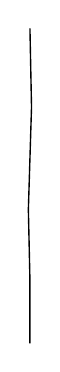
\begin{tikzpicture}\draw[line width=.5pt] (0,0)--(.02,-1)--(-.02,-2.3)--(0,-3.2)--(0,-4);\end{tikzpicture}}}}
\[
\operatorname{Pic}(X)\handwritten{\hookrightarrow}P(k)\ ,
\tag*{(22)}
\]
the obstruction for an element of $P(k)$ to beling to $\operatorname{Pic}(X)$\handwritten{(}being in $\operatorname{Br}\ H^{\unsure{o|0}}(X,\underline{O}_X)$, and hence\handwritten{)}vanishing if $k$ is algebraically \unsure{closed|closee}.
% archive sheet number: 10
\scanpage{12}
Here is a candidate for a functor, which may \unsure{tumn|turn} out to be representable, in which case this would be $P$. Let $\underline{A}$ be the ring-scheme over $k$ defined by $A$ (see Greenberg's papers, or Serre's in Bulletin Soc. Math.), so that
\[
A\handwritten{\simeq}\underline{A}(k)\ .
\tag*{(23)}
\]
For every algebra $B$ over $k$, corsider the ring $\underline{A}(B)$, which is an algebra over $\underline{A}(k)=A$. We may thus consider
\[
X_B\overset{\mathrm{dfn}}{=}X\handwritten{\otimes}_A\underline{A}(B)\ ,
\]
and consider the functor
\[
B\handwritten{\longmapsto}\operatorname{Pic}(X_B)\ .
\tag*{(\unsure{34|24})}
\]
This of course may not be representable, even if $A=k$. However, it may turn out that the fppf sheaf associated to this functor is representable, and this then would give the looked for cand\deleted{\unsure{r}}idate for $P$. In any case, Artin's work gives us a very handy set of necessary and sufficient conditions for a group functor to be representable by a scheme locally of finite type, and in principle it should be possible to decide wether or not the \deleted{functor} sheaf just considered satisfies to these conditions or not. If so, one may expect that the developments on local Picard schemes given for the case when there is a field of representatives will carry over to the case when the residue field is perfect with car.$\handwritten{>}0$.
% archive sheet number: 11
\scanpage{13}
In the construction of a local Picard scheme $Q$, we have seemed to use in a technically essential way the \deleted{fact} \inserted{assumption} that $U$ is regular (plus resolution). I would conjecture that a reasonable \unsure{loc al|local} Picard scheme $Q$, \inserted{locally of finite type over $k$,} can be constructed also without this assumption (provided that a field of representatives is given, \unsure{ar|or} the residue field is perfect of char. $p\handwritten{>}0$, of course). Instead of a resolution of singularities, one \unsure{\deleted{p}\handwritten{m}|$\mathbb{m}$}ay then wish to find a proper surjective morphism
\[
f:X\handwritten{\longrightarrow}S
\]
inducing an isomorphism $f^{-1}(U)\handwritten{\xrightarrow{\sim}}U$, and such that the corresponding map
\[
\operatorname{Pic}(X)\handwritten{\longrightarrow}\operatorname{Pic}(U)
\]
is \uline{surjective}. We then could repeat the construction of $P$, as $\lim\underline{\operatorname{Pic}}_{X_n/k}$, as above, and of $Q$ as $\operatorname{Coker}(\underline{D}\handwritten{\longrightarrow}P)$, where $\underline{D}$ is a group scheme corresponding to divisors concentrated on $X_o$ (possibly no longer discrete ?). Another way of approach would be to take a resolution of singularities $f:X\handwritten{\longrightarrow}S$, but where now we cannot assume any longer that $f^{-1}(U)\handwritten{\longrightarrow}U$ is an isomorphism, and to describe\deleted{\unsure{s}} a scheme $P$ in terms of invertible sheaves on $X$, together with \uline{descent data} of $\underline{L}\handwritten{|}f^{-1}(U)$ to $U$. A nice test for the yoga of local Picard schemes without regularity assumptions on $U$ would be to see if it is true in general that for $A$ Cohen-Macaulay of dim $\handwritten{\geq}3$ (more generally, for $H^2_{\underline{m}}(A)=0$), the group $\operatorname{Pic}(U)$ is indeed countable, and for separably closed residue field \deleted{\unsure{invariant}} \inserted{is invariant under} \uline{separable} field extension $k\handwritten{\longrightarrow}k'$, $A$ being replaced by $A\handwritten{\widehat{\otimes}}_k k'$ (which would express the expected \unsure{discrete|discreto} structure of the local Picard scheme).
% archive sheet number: 12
